\documentclass[12pt,a4paper,fleqn]{article}
\usepackage{rmpackages}																% usual packages
\usepackage{rmtemplate}																% graphic charter
\usepackage{rmexocptce}																% for DS with cptce eval

%\cfoot{} 													% if no page number is needed
%\renewcommand\arraystretch{1.5}		% stretch table line height

\usepackage{lscape}

\begin{document}
\normalem % makes emphasize italic again

\begin{header}
Chapitre 12 -- Actions mécaniques sur un système
\end{header}

\section{Actions mécaniques et forces}

Quand un objet agit sur un corps (le système), on dit que \textbf{l'objet exerce une action mécanique sur le système}.

\subsection{Le diagramme objet interactions}

Pour représenter cela, on peut utiliser un \textbf{diagramme objet interactions} :
\begin{itemize}
\item[•] on représente le \textbf{système} par un ovale ;
\item[•] on représente les \textbf{objets en interaction} avec le système par des rectangles ;
\item[•] on représente les interactions entre le système et les objets par des doubles flèches :
\begin{itemize}
\item avec des traits pleins quand il s'agit d'\textbf{actions de contact} (l'objet touche le système) ;
\item avec des traits pointillés quand il s'agit d'\textbf{actions à distance} (l'objet et le système ne se touchent pas).
\end{itemize} 
\end{itemize}

\begin{center}
\begin{tikzpicture}

\draw (0,0) node [bleu_f] {\textbf{Système}};
\draw [ultra thick, bleu_f] (0,0) ellipse (1.5cm and .5cm);

\draw (-2,2.5) node [red_f] {Objet 1};
\draw [ultra thick, red_f] (-3,2) rectangle++ (2,1);
\draw [<->, >=stealth, ultra thick, red_f] (0,.5) -- (-2,2);

\draw (4,1) node [green_f] {Objet 2};
\draw [ultra thick, green_f] (3,.5) rectangle++ (2,1);
\draw [<->, >=stealth, ultra thick, green_f, dashed] (1.5,0) -- (3,1);

\draw (-1,-2.5) node [red_f] {Objet 3};
\draw [ultra thick, orange_f] (-2,-3) rectangle++ (2,1);
\draw [<->, >=stealth, ultra thick, orange_f] (0,-.5) -- (-1,-2);
\end{tikzpicture}
\end{center}

\emph{On s'intéresse au système \{balle\}.
Construire un diagramme objet interaction dans chacune des trois situations du tableau ci-après.}

\subsection{Représentation des actions par des forces}

Pour représenter les actions mécaniques, on va utiliser le modèle des \textbf{forces}.
Pour chaque force, il faut déterminer :
\begin{itemize}
\item[•] son \textbf{point d'application}  :  le point où s'exerce la force ;
\item[•] sa \textbf{direction} : la droite selon laquelle s'exerce la force ;
\item[•] son \textbf{sens} : le sens de la force ;
\item[•] sa \textbf{norme} : proportionnelle à l'intensité de la force. 
\end{itemize}
On représente donc une force par un \blank{vecteur}.

\emph{Pour chaque situation, représenter les forces s'exerçant sur le système.}

\newpage


\begin{landscape}
\begin{center}
\begin{tabular}[c]{|c| >{\centering}m{.3\linewidth} | >{\centering\arraybackslash}m{.3\linewidth} |}
\hline
\textbf{Situation} & \textbf{Diagramme objet interaction} & \textbf{Forces} \\
\hline
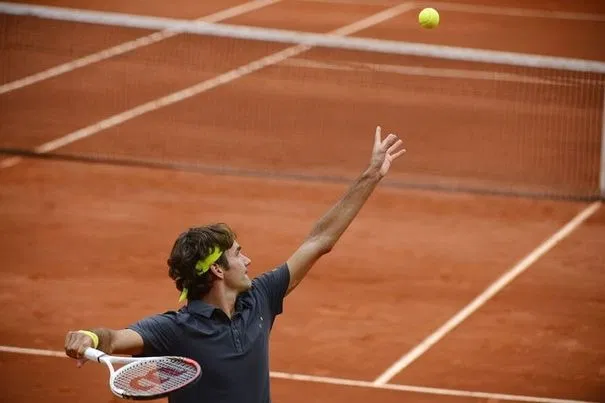
\includegraphics[trim=0 0 50 -13, clip, width=200pt]{images/tennis_service.png} & & \\
\hline
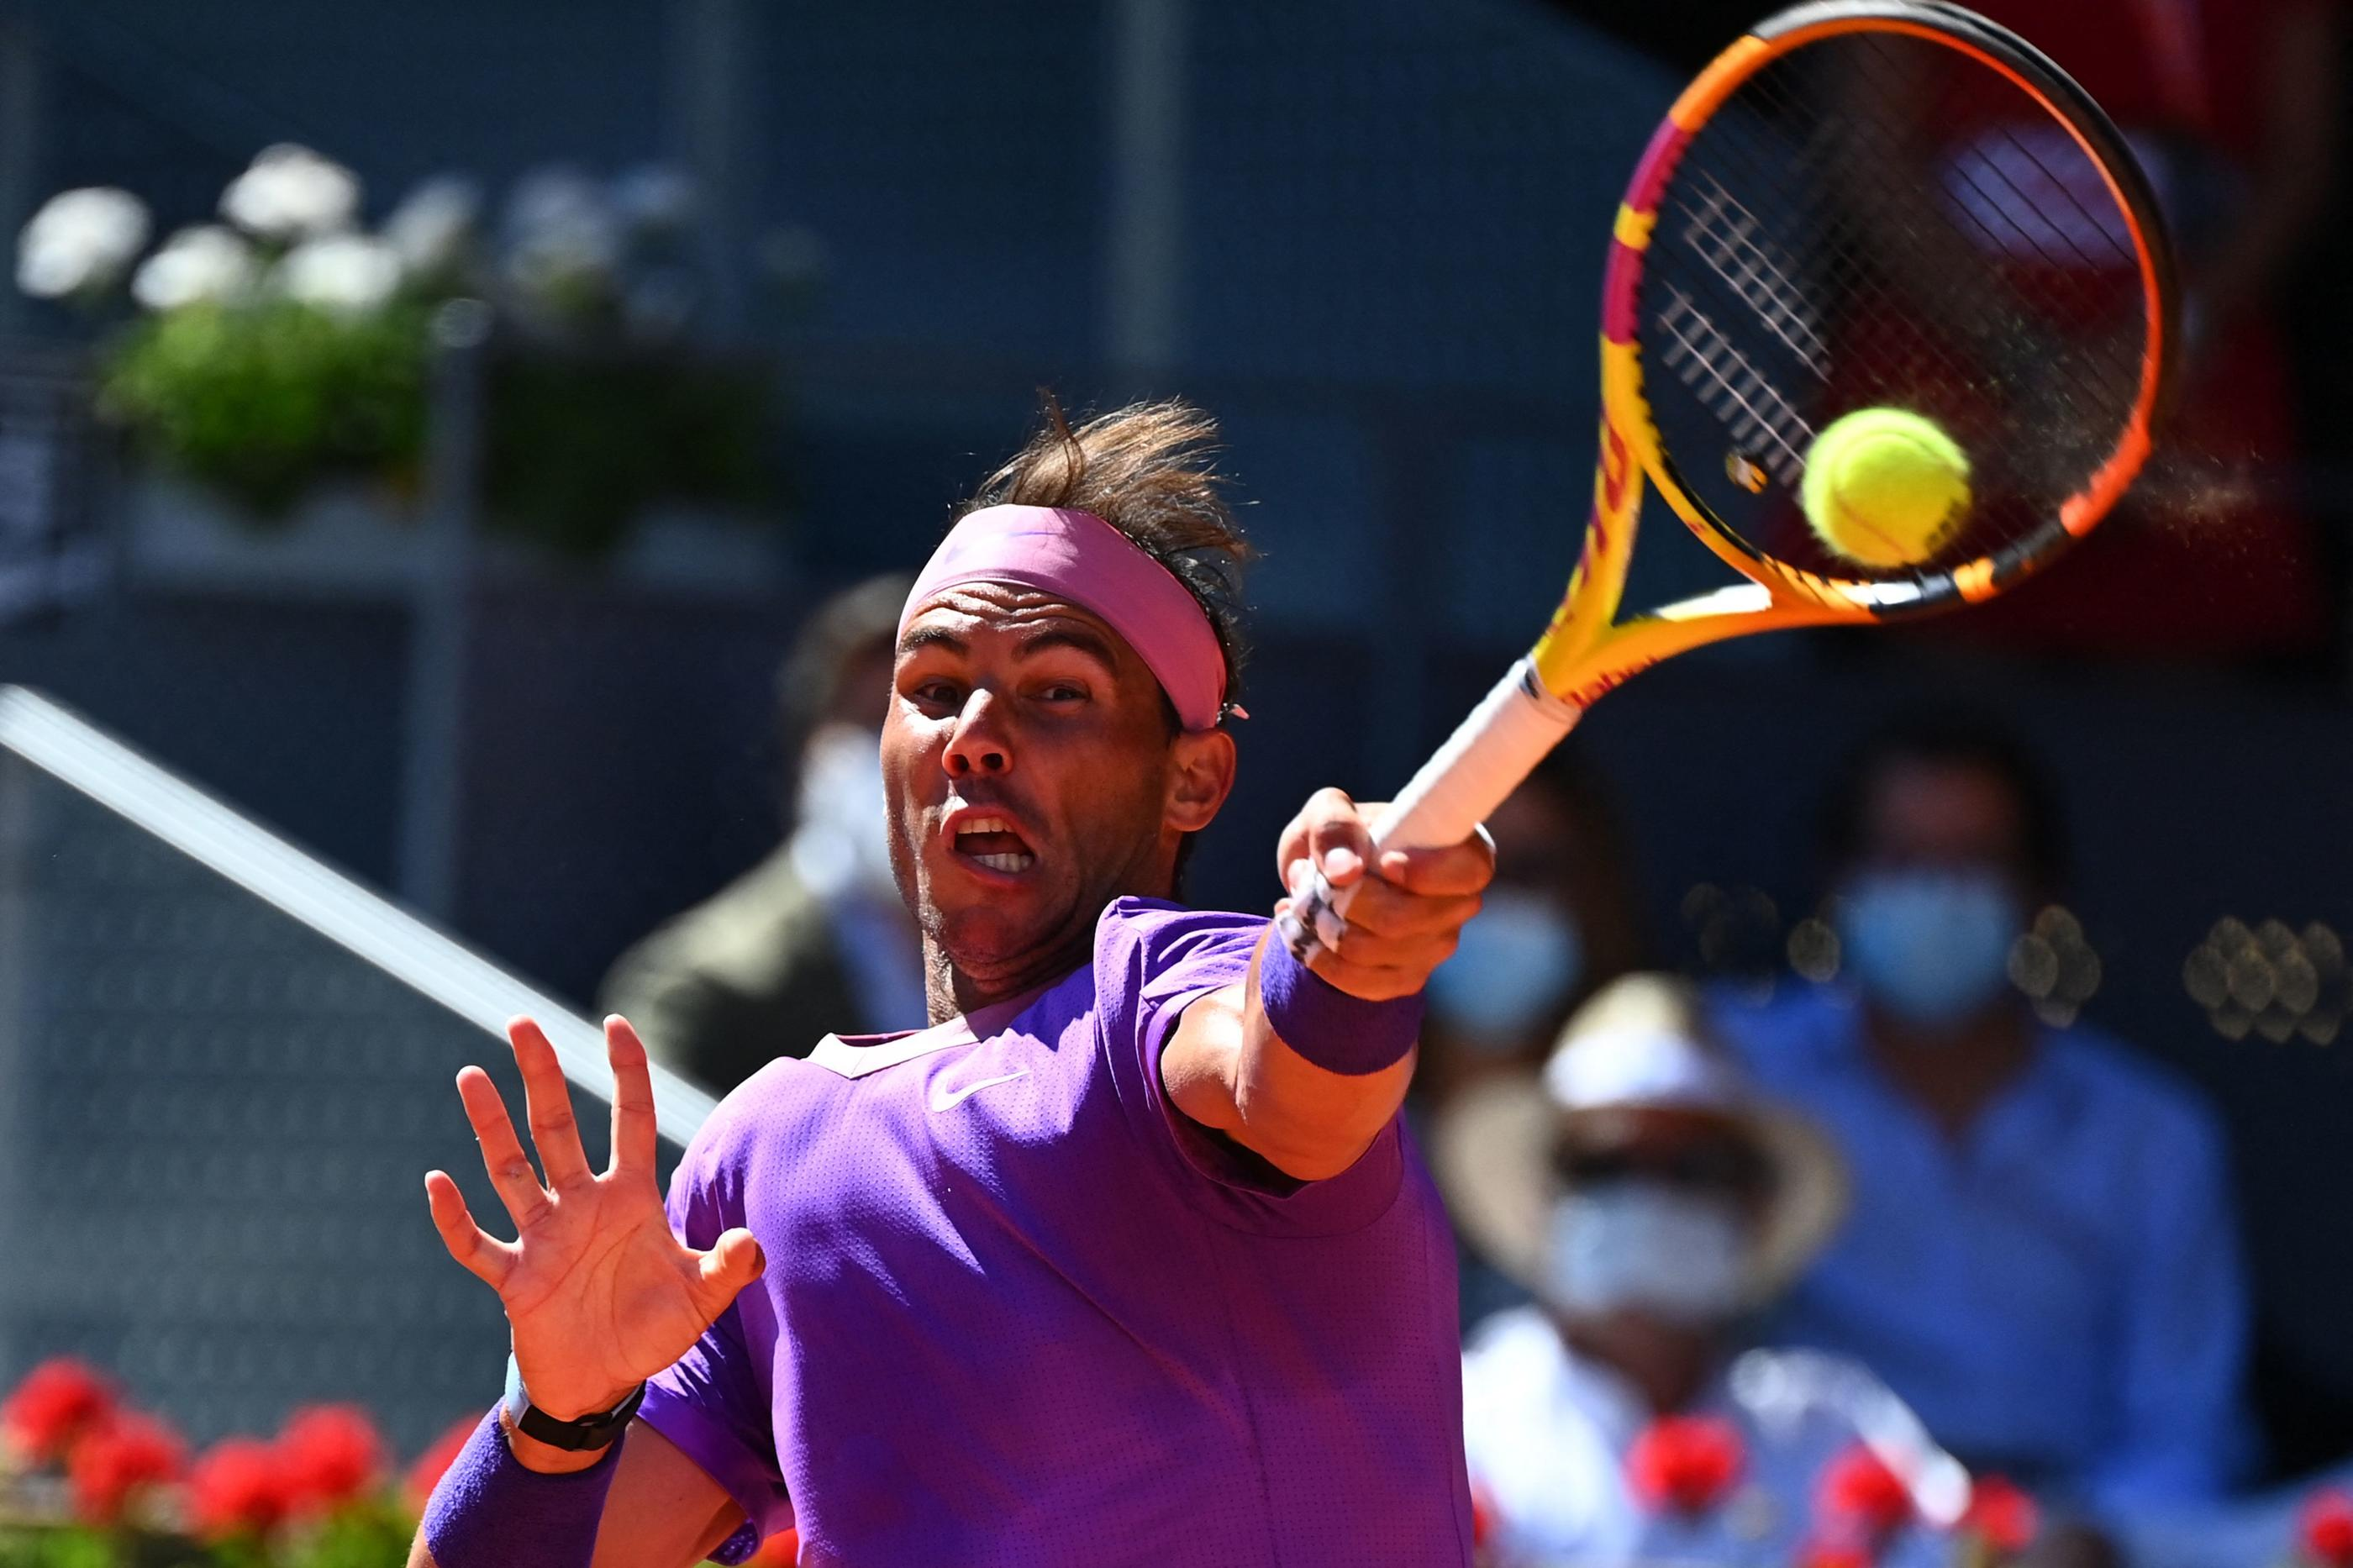
\includegraphics[trim=50 0 0 -13, clip, width=200pt]{images/tennis_raquette.jpg} & & \\
\hline 
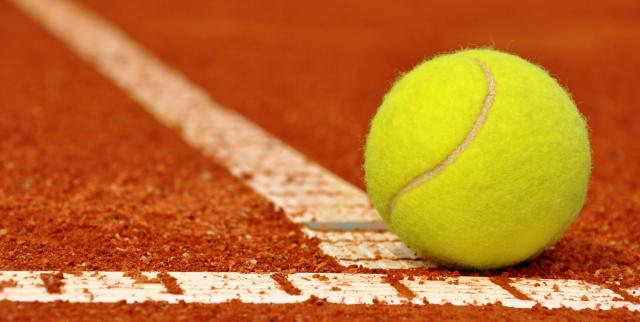
\includegraphics[trim=125 0 0 -8, clip, width=200pt]{images/tennis_sol.jpg} & & \\
\hline
\end{tabular}
\end{center}
\end{landscape}

\section{Quelques forces à connaitre}

Toutes les forces s'expriment en \textbf{newton} (\textbf{N}).

\subsection{Force d'interaction gravitationnelle (exemple Soleil-Terre)}

\textbf{Deux corps massifs s'attirent !}

\begin{center}
\begin{tikzpicture}
\coordinate (O) at (0,0);
\shade[ball color = yellow_f, opacity = .5] (O) circle (1);
\node at (O) [above left] {$S$};
\node at (O) {$\bullet$};

\coordinate (M) at (6,2);
\shade[ball color = bleu_f] (M) circle (.25);
\node at (M) [above left] {$T$};
\node at (M) {$\bullet$};

\draw [dashed] (O) -- (M) node [midway, above] {$d$};

\draw [ultra thick, red_f, -stealth] (O) --++ (1.5,.5) node [midway, below right] {$\vec{F}_\mathrm{T/S}$};
\draw [ultra thick, red_f, -stealth] (M) --++ (-1.5,-.5) node [midway, above left] {$\vec{F}_\mathrm{S/T}$};
\end{tikzpicture}
\end{center}

\paragraph{Caractéristiques de la force d'interaction gravitationnelle : $F_\mathrm{G}$}
\begin{itemize}
\item[•] point d'application : centre du système ;
\item[•] direction : droite $(ST)$ ;
\item[•] sens : vers l'autre objet ;
\item[•] norme : elle s'exprime à l'aide la constante gravitationnelle ($G = \qty[per-mode=power, inter-unit-product=\cdot]{6,67e-11}{\meter\cubed\per\kilogram\per\second\squared}$) et dépend de la masse des deux objets exprimée en kilogrammes ($M_\odot$ pour le Soleil et $M_\mathrm{T}$ pour la Terre) et de la distance $d$ entre le centre des deux objets, exprimée en mètres :
\[F_\mathrm{G} = G \times \frac{M_\odot \times M_\mathrm{T}}{d^2}\]
\end{itemize}

\subsection{Poids (exemple d'une balle de tennis}

\textbf{Un corps massif est attiré par la Terre !}
Mais on l'a déjà dit ça non ?
Si !

\begin{center}
\begin{tikzpicture}
\draw (0,0) -- (6,0);
\foreach \x in {0,0.25,...,6} {
    \draw (\x, 0) --++ (-.25, -.25);
}
\coordinate (M) at (3,2);
\shade[ball color = yellow_f] (M) circle (0.5);
\draw [ultra thick, red_f, -stealth] (M) --++ (0,-1) node [midway, below right] {$\vec{P}$};
\end{tikzpicture}
\end{center}

\paragraph{Caractéristiques du poids : $P$}
\begin{itemize}
\item[•] point d'application : centre du système
\item[•] direction : verticale
\item[•] sens : vers le bas
\item[•] norme : $P = m \times g$ où $m$ est la masse du système et $g$ est l'accélération de pesanteur ($g=\qty[per-mode=power, inter-unit-product=\cdot]{9,81}{\meter\per\second\squared}$).
\end{itemize}

\paragraph{Remarque :}
Le poids n'est qu'une réécriture de la force d'interaction gravitationnelle !
On peut s'en convaincre en calculant la force d'interaction gravitationnelle entre la balle et la Terre et le poids de la balle.
Lors de l'étude du mouvement d'un projectile proche du sol, on utilise le poids alors que pour le mouvement d'un satellite, il faut utiliser la force d'interaction gravitationnelle.


\newpage
\subsection{Force exercée par un support (exemple : balle posée par terre)}

\begin{center}
\begin{tikzpicture}
\draw (0,0) -- (6,0);
\foreach \x in {0,0.25,...,6} {
    \draw (\x, 0) --++ (-.25, -.25);
}
\coordinate (M) at (3,0.75);
\shade[ball color = yellow_f] (M) circle (0.75);
\draw [ultra thick, red_f, -stealth] (3,0) --++ (0,2) node [midway, left] {$\vec{R}$};
\end{tikzpicture}
\end{center}
\emph{Le poids n'est pas représenté sur le schéma mais il s'exerce toujours sur la balle.}

\paragraph{Caractéristiques de la réaction du support : $R$}
\begin{itemize}
\item[•] point d'application : point de contact entre le système et le support ;
\item[•] direction : ça dépend (ici, verticale car la balle est immobile et le support horizontal) ;
\item[•] sens : ça dépend, mais plutôt vers le système ;
\item[•] norme : ça dépend (ici, $R=P$ pour les mêmes raisons qu'auparavant).
\end{itemize}

\subsection{Force exercée par un fil (une balle suspendue à un fil : le pendule)}

\begin{center}
\begin{tikzpicture}
\draw (-3,0) -- (3,0);
\foreach \x in {0,0.25,...,6} {
    \draw (\x-3, 0) --++ (.25, .25);
}
\coordinate (M) at (-60:4);
\draw (O) -- (M);
\shade[ball color = yellow_f] (M) circle (0.5);
\draw [ultra thick, red_f, -stealth] (M)++(120:0.5) --++ (120:1) node [midway, right] {$\vec{T}$};
\end{tikzpicture}
\end{center}

\emph{Le poids n'est pas représenté sur le schéma mais il s'exerce toujours sur la balle.}

\paragraph{Caractéristiques de la réaction du support : $R$}
\begin{itemize}
\item[•] point d'application : point de contact entre le système et le fil ;
\item[•] direction : celle du fil ;
\item[•] sens : à l'opposé du système ;
\item[•] norme : ça dépend (ici, il faut faire le calcul...).
\end{itemize}

\section{Principe des actions réciproques}

Lorsque deux objets sont en interaction, ils exercent l'un sur l'autre des forces opposées.
Ces forces ont : 
\begin{itemize}
\item[•] la même direction ;
\item[•] des sens opposés ;
\item[•] la même norme.
\end{itemize}
Ce principe est valable aussi bien pour les actions à distance que pour les actions de contact.

\end{document}